
La idea de random forest es utlizar múltiples árboles de decisión para mejorar la eficacia del clasificador, reduciendo la alta varianza que se observa en la utilización de un único árbol. Esto es posible gracias al bajo costos que lleva entrenar y consultar a cada árbol. 
 La reducción en la varianza suele ser mas significativa cuando el bosque se arma con árboles que utilicen diferentes atributos. Para lograr esto los atributos utilizados en las divisiones de los nodo al construir el árbol se limitan a un subconjunto aleatorio de los atributos, reduciendo la probabilidad que lo atributos con mayor ganancia de información dominen todos los arboles. 
Utilizando los mismos parámetros que para el clasificador de un único árbol volvimos a hacer pruebas variando la cantidad de árboles del bosque y el tamaño del subconjunto de atributos a considerar. En la figura ~\ref{fig:forest_f05_en_funcion_de_cantidad_de_arboles} se muestran los resultados para bosques de diferentes tamaños considerando n, $\sqrt{n}$ y $\log(n)$ atributos, donde n es la cantidad total de atributos. Los bosques en loas cuales se consideran n atributos muestran mejores resultados, pero cuando consideran $\sqrt{n}$ atributos, la varianza es inferior por lo que esperamos que la eficacia con datos nuevos sea más parecida a lo  que observamos con cross validation sobre datos de entrenamiento. 


\begin{figure}[H]
  \centering
  \begin{minipage}[b]{0.45\textwidth}
    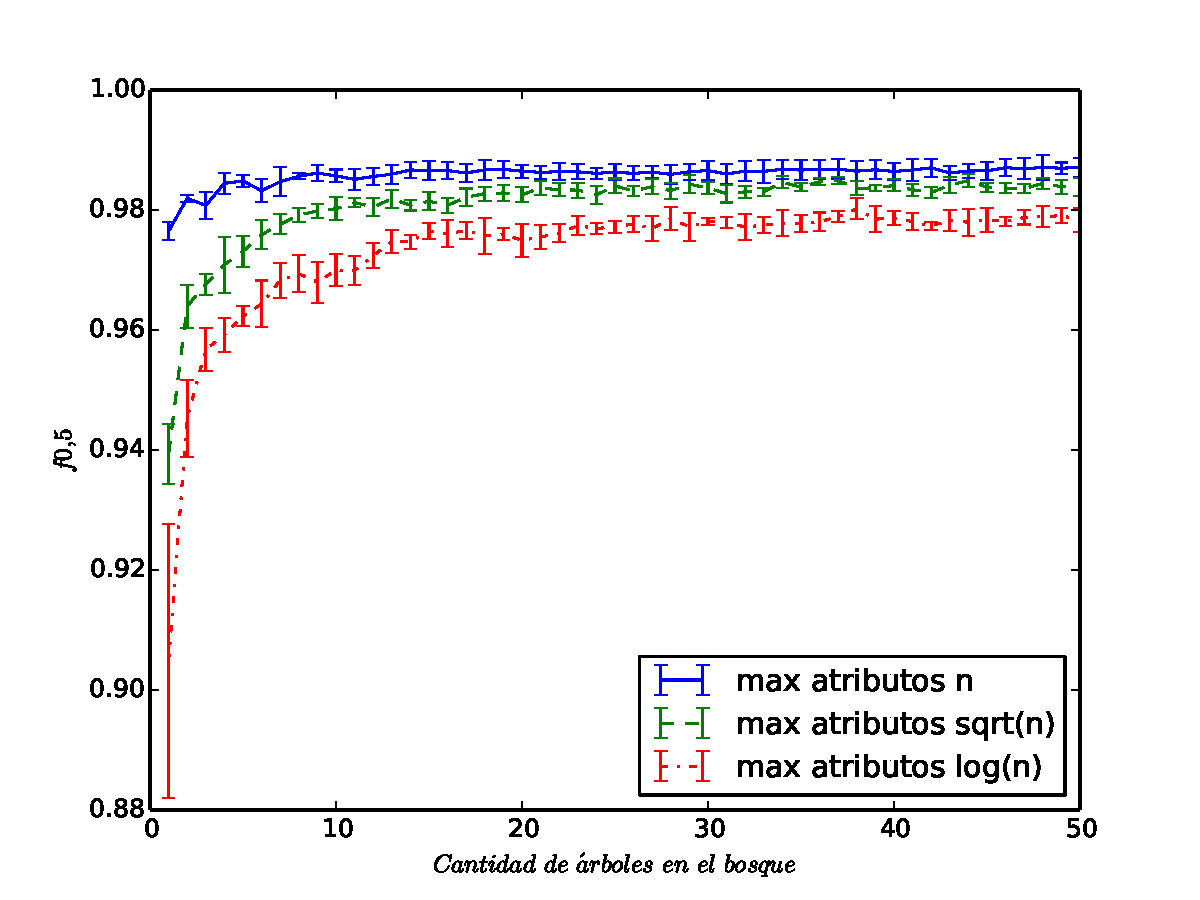
\includegraphics[width=\textwidth]{plots/random_forest.pdf}
    \caption{$f_{0.5}$ en función de la cantidad de árboles}
  \end{minipage}
  \hfill
  \begin{minipage}[b]{0.45\textwidth}
    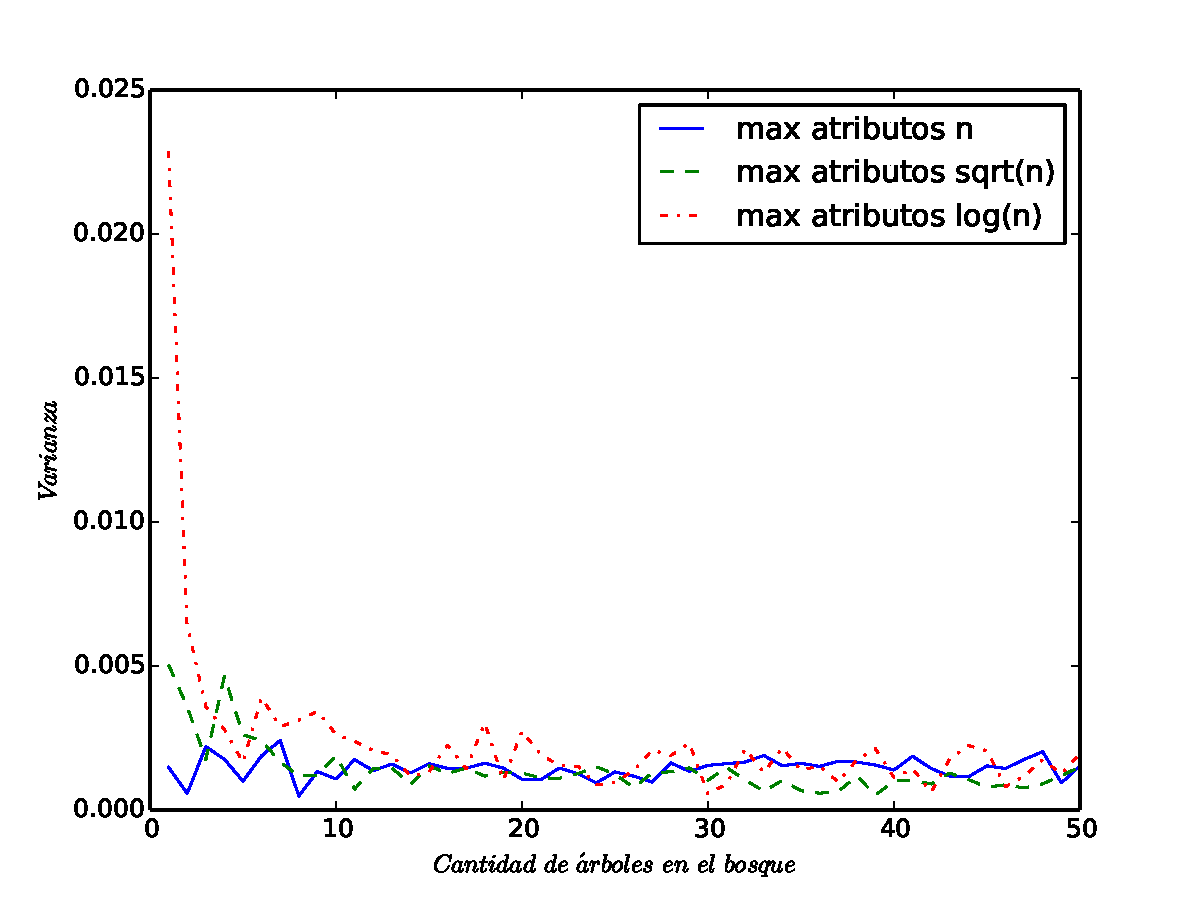
\includegraphics[width=\textwidth]{plots/random_forest_var.pdf}
    \caption{Varianza en función de la cantidad de árboles}
  \end{minipage}
  \label{fig:forest_f05_en_funcion_de_cantidad_de_arboles}
\end{figure}